%*****************************************************************************************
%********************************** Fourth Chapter ***************************************
%*****************************************************************************************

\chapter{MHD Waves excited by Different Photospheric Driver Profiles}

\begin{pycode}[chapter4]
ch4 = texfigure.Manager(pytex, number=4, base_path='./Chapter4/')
\end{pycode}

%%{\Large Knowledge at start:}
%%\begin{itemize}
%%	\item The ideal MHD equations
%%	\item Wave solutions for a uniform media
%%	\item velocity perturbation calculations
%%	\item Wave flux calcs
%%	\item SAC, and numerical solutions to the ideal MHD equations
%%	\item Static background conditions
%%	\item Construction of flux surfaces
%%	\item The specific numerical domain used for all the simulations.
%%\end{itemize}

\section{Driving Waves from the Photosphere}\label{sec:5drivers}

As discussed in \cref{ch:Background} the plasma conditions in the photosphere are conducive to the generation of MHD waves.
The photosphere is seeded with small scale magnetic features and dynamic plasma motions as a result of the granulation.
In this chapter the motions that are common in the inter-granular lanes will be studied for their potential ability to drive MHD waves in small scale magnetic flux tubes.
Considering the physical conditions of the inter-granular lanes, where parcels of hot plasma rise, expand and then sink down these lanes.
It is easy to imagine the motions present: vertical motion caused by rising and sinking plasma; horizontal motion caused by the expansion and contraction of the plasma as it cools; spiralling motion in which plasma sinks down magnetic field lines, analogous to that of water down a plug hole.

The horizontal and vertical motions are commonly observed using high resolution observations, the spiralling motions were observed in an inter-granular lane by \cite{Bonet2008} and various types of spirals have been observed in the higher layers of the atmosphere by \cite{Wedemeyer-Bohm2009,Wedemeyer-Bohm2012,Wedemeyer2013}.
The different types of spiral observed in the atmosphere and the difficulty of performing high quality observations of plasma motions in the inter-granular lanes, the spiralling motions will be modelled by a variety of drivers.
A circular driver, a `spiral' with no radial (expansion) component; an Archemedian spiral, a spiral which expands by a fixed amount for each rotation; and a logarithmic spiral where the spiral expands by an exponentially increasing amount with every rotation.

To drive waves in the numerical domain described in \cref{ch:Background} the plasma has to be `moved' by numerically adding a velocity field to the domain.
This is done by adding the desired velocity field to a 3D layer close to the bottom of the domain, within the modelled photosphere.
This velocity field is attenuated with a Gaussian profile in three dimensions and is located at the centre of the domain aligned with the foot point of the magnetic field.
This velocity field is then multiplied by a sine function to make it periodic. The generic form of the driver is given in \cref{eq:generic_driver}.
\begin{equation}
	V(x,y,z) = F(x,y,z) \ e^{-\left(\frac{z^2}{\Delta z^2} + \frac{x^2}{\Delta x^2} + \frac{y^2}{\Delta y^2}\right)} \sin \left(2\pi \frac{t}{P}\right),
	\label{eq:generic_driver}
\end{equation}
where, $V(x,y,z)$ is the output velocity field, $F(x,y,x)$ is an arbitrary function which defines the form of the driver, $\Delta x$, $\Delta y$, $\Delta z$ are the widths of the Gaussian function in the three spatial dimensions, and $P$ is the period of the driver.
The values used for the width of the Gaussians are fixed through out this thesis and are: $\Delta x = \Delta y = 0.1$ Mm and $\Delta z = 0.05$, the origin of the driver is at $z = 100$ km above the photosphere.

The five driving motions, horizontal, vertical, circular, Archemedian spiral and logarithmic spiral are then defined by the form of $F(x,y,z)$. For the horizontal and vertical drivers $F(x,y,z)$ is a constant in the direction of the motion, $x$ for horizontal and $z$ for vertical, for the spiral drivers the forms of $F(x,y,z)$ are given in \cref{eq:Suni,eq:Sarch,eq:Slog}.

\begin{subequations}
	\begin{align}
		F(x) &= A \frac{y}{\sqrt{x^2 + y^2}}\\
		F(y) &= - A \frac{x}{\sqrt{x^2 + y^2}},
	\end{align}
	\label{eq:Suni}
\end{subequations}
 
\begin{subequations}
	\begin{align}
		F(x) &= A \frac{\cos(\theta + \phi)}{\sqrt{x^2 + y^2}},\\
		F(y) &= - A \frac{\sin(\theta + \phi)}{\sqrt{x^2 + y^2}},\\
			&\text{where}\notag\\
			&\theta = \tan^{-1}\left(\frac{y}{x}\right),\ \phi = \tan^{-1}\left(\frac{1}{B_L}\right).\notag	
	\end{align}
	\label{eq:Slog}
\end{subequations}
and $B_L = 0.05$ and is a dimensionless expansion parameter for the logarithmic spiral.
 
\begin{subequations}
	\begin{align}
		F(x) &= A \frac{B_Ax}{x^2 + y^2} \frac{y}{\sqrt{x^2 + y^2}},\\
		F(y) &= - A \frac{B_Ay}{x^2 + y^2} \frac{x}{\sqrt{x^2 + y^2}},
	\end{align}
	\label{eq:Sarch}
\end{subequations}
$B_A = 0.005$ is similar in nature to $B_L$, \textit{i.e.} a dimensionless expansion parameter.
The amplitude $A$ of all the drivers is set to $10$ ms$^{-1}$ for all the simulations performed in this chapter and the period is fixed at $240$ s.
Visualisations of these velocity fields can be seen in \cref{fig:spiral_driver_cut}.


\begin{pycode}[chapter4]
from streamlines import Streamlines
#Use Equation 1 to calculate the vector field in a 2D plane to plot it.
time = np.linspace(0,60,480)
dt = time[1:] - time [:-1]
period = 240.

x = np.linspace(7812.5,1992187.5,128)
y = np.linspace(7812.5,1992187.5,128)

x_max = x.max()
y_max = y.max()

xc = 1.0e6
yc = 1.0e6

xn = x - xc
yn = y - yc

delta_x=0.1e6
delta_y=0.1e6

xx, yy = np.meshgrid(xn,yn)
exp_y = np.exp(-(yn**2.0/delta_y**2.0))
exp_x = np.exp(-(xn**2.0/delta_x**2.0))

exp_x2, exp_y2= np.meshgrid(exp_x,exp_y)
exp_xyz = exp_x2 * exp_y2


#==============================================================================
# Define Driver Equations and Parameters
#==============================================================================
#A is the amplitude, B is the spiral expansion factor
A = 10

#Tdamp defines the damping of the driver with time, Tdep is the ocillator
tdamp = lambda time1: 1.0 #*np.exp(-(time1/(period)))
tdep = lambda time1: np.sin((time1*2.0*np.pi)/period) * tdamp(time1)

#Define a peak index to use for scaling in the inital frame
max_ind = np.argmax(tdep(time) > 0.9998)

def log():
	B = 0.05
	phi = np.arctan2(1,B)
	theta = np.arctan2(yy,xx)
	
	uy = np.sin(theta + phi)
	ux =  np.cos(theta + phi)
	
	vx = lambda time1: (ux / np.sqrt(ux**2 + uy**2)) * exp_xyz * tdep(time1) * A
	vy = lambda time1: (uy / np.sqrt(ux**2 + uy**2)) * exp_xyz * tdep(time1) * A
	
	vv = np.sqrt(vx(time[max_ind])**2 + vy(time[max_ind])**2)
	
	return vx, vy, vv

def arch():
	B = 0.005
	r = np.sqrt(xx**2 + yy**2)
	
	vx = lambda time1: ( (B*1e6 * xx) / (xx**2 + yy**2) + yy/r ) * exp_xyz * tdep(time1) * A
	vy = lambda time1: ( (B*1e6 * yy) / (xx**2 + yy**2) - xx/r ) * exp_xyz * tdep(time1) * A
	
	vv = np.sqrt(vx(time[max_ind])**2 + vy(time[max_ind])**2)
	
	return vx, vy, vv

def uniform():
    #Uniform
    vx = lambda time1: A * (yy / np.sqrt(xx**2 + yy**2)) * exp_xyz * tdep(time1)
    vy = lambda time1: A * (-xx / np.sqrt(xx**2 + yy**2)) * exp_xyz * tdep(time1)
    vv = np.sqrt(vx(time[max_ind])**2 + vy(time[max_ind])**2)
    
    return vx, vy, vv

drivers = [log, arch, uniform]

driver_figs = texfigure.MultiFigure(3, 2, reference='driver_figs')
for driver_func in drivers:
    fig, ax = plt.subplots()
    #============================================================================
    # Do the Plotting
    #============================================================================
    vx, vy, vv = driver_func()
    # Calculate Streamline
    slines = Streamlines(x,y,vx(time[max_ind]),vy(time[max_ind]),maxLen=7000,
                         x0=xc, y0=yc, direction='forwards')

    im = ax.imshow(vv, cmap='Blues', extent=[7812.5,x_max,7812.5,y_max])
    im.set_norm(matplotlib.colors.Normalize(vmin=0,vmax=A))
    #ax.hold()
    
    if driver_func != uniform:
        Sline, = ax.plot(slines.streamlines[0][0],slines.streamlines[0][1],color='red',linewidth=2, zorder=40)
    else:
	    Sline = matplotlib.patches.Circle([1e6, 1e6], radius=.15e6, fill=False, color='red', linewidth=2, zorder=40)
	    ax.add_artist(Sline)

    #Add colourbar
    divider = make_axes_locatable(ax)
    cax = divider.append_axes("right", size="5%", pad=0.2)
    cbar = plt.colorbar(im,cax)
    cbar.set_label(r"$|V|$ [ms$^{-1}$]")
    scalar = matplotlib.ticker.ScalarFormatter(useMathText=False,useOffset=False)
    scalar.set_powerlimits((-3,3))
    cbar.formatter = scalar
    cbar.ax.yaxis.get_offset_text().set_visible(True)
    cbar.update_ticks()
    #cbar.solids.set_rasterized(True)
    cbar.solids.set_edgecolor("face")

    #Add quiver plot overlay
    qu = ax.quiver(x,y,vx(time[max_ind]),vy(time[max_ind]),scale=25*A,color='k',zorder=20, linewidth=1)
    ax.axis([8.0e5,12.0e5,8.0e5,12.0e5])

    ax.xaxis.set_major_formatter(scalar)
    ax.yaxis.set_major_formatter(scalar)
    ax.xaxis.set_major_locator(matplotlib.ticker.MaxNLocator(5))
    ax.yaxis.set_major_locator(matplotlib.ticker.MaxNLocator(5))
    ax.xaxis.get_offset_text().set_visible(False)
    ax.yaxis.get_offset_text().set_visible(False)
    ax.set_xlabel("X [Mm]")
    ax.set_ylabel("Y [Mm]")

    plt.tight_layout()
    Fig = ch4.save_figure(driver_func.__name__, fig)
    driver_figs.append(Fig)

driver_figs.figures[0,0].caption = "Archemdian spiral velocity field with expansion factor $B_A=0.005$"
driver_figs.figures[0,1].caption = "Logarithmic spiral velocity field with expansion factor $B_L=0.05$"
driver_figs.figures[1,0].caption = "Uniform spiral velocity field"

driver_figs.caption = "Horizontal cuts through the spiral driver at the peak amplitude height $z = 0.01$ Mm for the two spiral drivers. Red lines are a streamline of the velocity vector field, sampled as black arrows, overplotted on the velocity magnitude $|V|$."
\end{pycode}

\py[chapter4]|driver_figs|

\section{Simulations}

Five different simulations, one for each driver profile shown in \cref{fig:driver_figs}, were performed using the SAC code as described in \cref{sec:SAC}.
These simulations were performed using the background conditions described in \cref{sec:mhsbackground} on a $128^3$ grid with physical dimensions of $2.0 \times\ 2.0\ \times\ 1.6$ Mm$^3$ in the $x$, $y$ and $z$ directions respectively, and with an origin in the $z$ direction of $0.061$ Mm above the photosphere.
The plasma was driven using the different drivers described in \cref{sec:5drivers} continuously for the length of the simulations. 
%TODO: What length are we showing here?

Snapshots of one of the simulations are shown as 3D renders in \cref{fig:frames_Suni_vphi}, the driving velocity field is represented as vectors at the base and the flux surface is shown, coloured with the azimuthal velocity component.

\begin{figure}[h]
    \begin{subfigure}[b]{0.9\columnwidth}
        \centering
        \includegraphics[width=0.55\columnwidth]{Chapter4/Figs/Mayavi_Slog_p240_A10_r60_vphi_00150.png}
        \caption{Snapshot at $t=154$ s}
    \end{subfigure}
    \begin{subfigure}[b]{0.9\columnwidth}
        \centering
        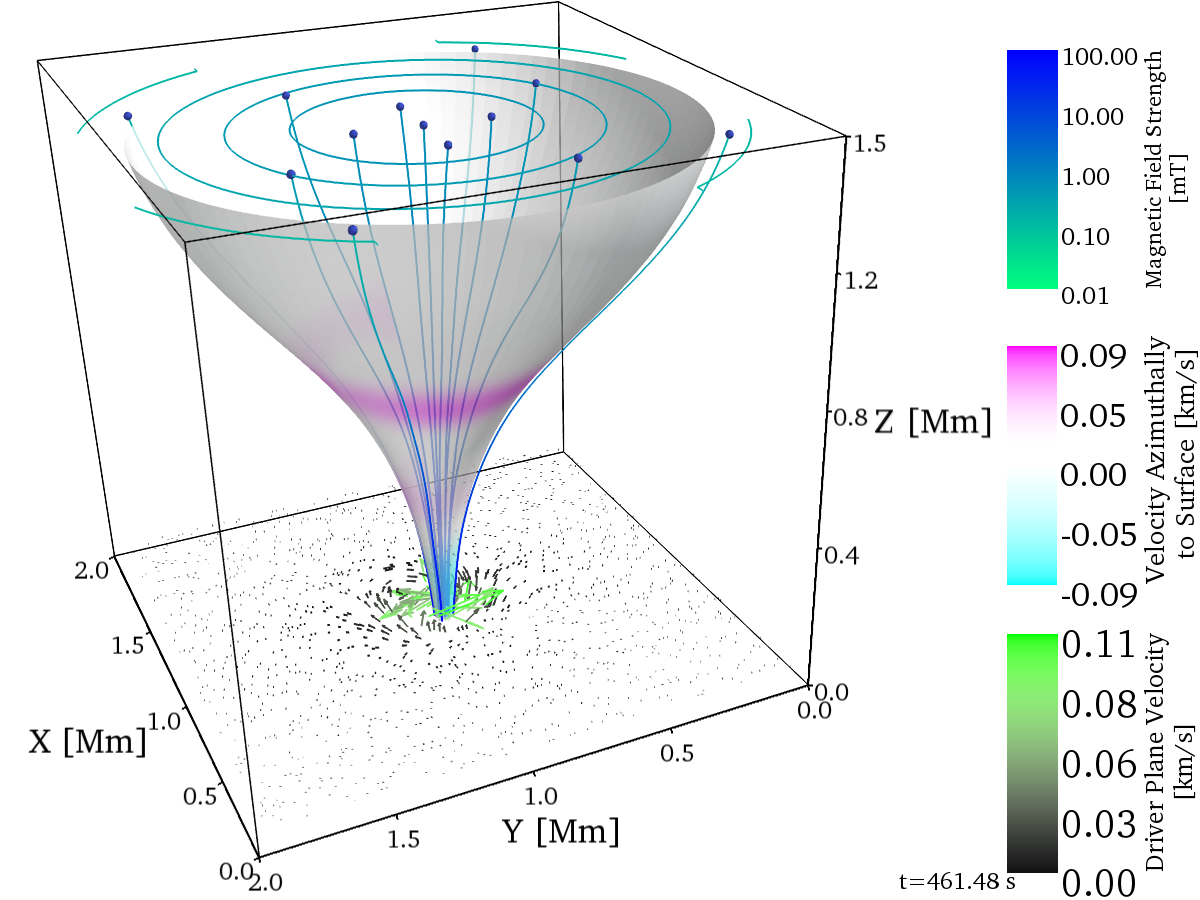
\includegraphics[width=0.55\columnwidth]{Chapter4/Figs/Mayavi_Slog_p240_A10_r60_vphi_00450.png}
        \caption{Snapshot at $t=461$ s}
    \end{subfigure}
    \begin{subfigure}[b]{0.9\columnwidth}
        \centering
        \includegraphics[width=0.55\columnwidth]{Chapter4/Figs/Mayavi_Slog_p240_A10_r60_vphi_00586.png}
        \caption{Snapshot at  $t=600$ s}
    \end{subfigure}
    \caption{Snapshots at three time steps of a 3D render of the simulation domain for the logarithmic spiral driver with a flux tube radius of $r = 936$ km (at the top of the computational domain). Shown in the domain are magnetic field lines and field strength contours in cyan, as well as the velocity vector field at the peak height of the driver shown as green and black arrows at the base, and the reconstructed surface coloured with the azimuthal velocity component ($V_\phi$).}
    \label{fig:frames_Suni_vphi}
\end{figure}

\subsection{Comparing Wave Excitation}

As described in \cref{sec:fluxsurfaces} flux surfaces can be used to analyse the relative properties of the major MHD modes in a system.
In this section we will apply this analysis method to the simulations of various drivers.

The results of applying the analysis which is discussed in Sect. \ref{sec:3d_analysis} are shown in Fig. \ref{fig:frames_Suni_vphi}, as snapshots at times $154$, $461$ and $600 \text{ s}$ of wave propagation along the magnetic flux tube surface as generated by a logarithmic spiral driver (see Equation \ref{eq:Slog}) with a period of $240$ s.
In Fig. \ref{fig:frames_Suni_vphi} it can be seen that the torsional driver excites perturbations in each decomposed velocity component, \textit{e.g.} $V_\phi$,  $V_\perp$, $V_\parallel$, as would be expected for a driver that is not exactly a linear eigenmode of the system. 
The strength and positions of these perturbations change as the simulations progress and the wave fronts travel along the tube. 
Also shown is a vector plane at the peak vertical height of the driver, which illustrates the velocity field driving the oscillations.
To analyse the propagation of separate wave modes we extracted the velocity components along a magnetic field line on the flux surface and constructed time-distance diagrams for each component. 
One magnetic field line is chosen at the beginning of the simulation and the values on the polygons between this field line and an adjacent field line are extracted for each time-step and presented in the time-distance diagrams in Fig. \ref{fig:All_TD_wave_30}. 
The perturbations are assumed to be linear, as no correction is made for the (vertical) movement of the surface itself. 
This assumption is verified by calculating the variation in the coordinates for the polygons at each time-step and it is found to be substantially less than one grid point for all the results presented here.

\subsubsection{Mode Identification}
To identify the observed MHD wave modes we shall initially consider the phase speed of the perturbations in the time-distance diagrams. 
In our numerical domain, both inside and outside the flux tube, there is plasma $\beta > 1$.
In analysing the results we identified the fast sausage mode, the slow kink mode and the Alfv\'en mode.
To aid in the analysis of Fig. \ref{fig:All_TD_wave_30} overplotted are the Alfv\'en speed $v_A$ and sound speed $c_s$, as well as the speed of the fast magneto-acoustic wave (fast speed) $v_f^2 = \sqrt{c_s^2 + v_A^2}$ and the slow speed (or tube speed) $v_t^{-2} = \sqrt{c_s^{-2} + v_A^{-2}}$ for the equilibrium background, starting at $60$ s, the first peak of the driver amplitude. 
It should be noted that this analysis is still an approximation of our simulated system because we have non-constant, non-uniform, non-straight magnetic field in a stratified solar atmosphere, where one would expect the observed phase speed to deviate from these first-order estimations, as can be seen in Fig. \ref{fig:All_TD_wave_30}.

First, we take the case of the horizontal driver, Fig. \ref{fig:All_TD_wave_30:horiz}, in the most detail. 
In the $V_\parallel$ component we expect to see the fast sausage mode being the dominant mode, which is observed.
There is also a weaker presence of a perturbation with the phase speed closer to that of the Alfv\'en and slow speeds but offset from the starting point of the over-plotted lines; This is attributed to the coupling of the wave modes in our non-homogeneous plasma.
In the $V_\perp$ component the presence of a slow kink mode travelling close to the tube speed $v_t$ (solid line).
This mode is the dominant contribution in this panel and is approximately two times stronger when compared the perturbations in the parallel component. 
Finally, the azimuthal velocity component ($V_\phi$) has a very small contribution, of an order of magnitude less, travelling at the Alfv\'en speed, which we attribute to our driver not being perfectly centred upon the flux tube axis.

Comparing the results of the wave excitation by the vertical periodic driver to that of the horizontal driver, it is easy to draw parallels in the description.
However, there are some key differences. 
In this case, of wave excitation by the vertical driver, most of the perturbation is in the $V_\parallel$ velocity component, with a much stronger contribution from the fast sausage mode ($\approx 20 \times$ stronger than $V_\perp$).
There is also evidence of a rapidly spatially damped mode observed in the top panel of Fig. \ref{fig:All_TD_wave_30:vert}.
This spatial damping is attributed to the expansion of the magnetic flux tube, and the dispersion of the wave energy over a wider volume as the tube expands.
The $V_\perp$ component on the vertical driver's time-distance diagram is very weak, with only a weak fast kink mode component easily visible, apart from some small reflection from the top boundary. 
Finally, the vertical driver's $V_\phi$ component is, like its horizontally driven $V_\phi$ counterpart, substantially weaker than the other two components.

Next, we analyse the results of the three simulations with torsional drivers.
The time-distance diagrams for the three different torsional drivers have similar properties; the vast majority of the perturbation for all the torsional drivers is, as expected, in the $V_\phi$ component.
The other two components are of an order of magnitude less than the values of $V_\phi$.
The time-distance diagrams for the uniform torsional and the Archimedean spiral driver, Figs. \ref{fig:All_TD_wave_30:Suni} \& \ref{fig:All_TD_wave_30:Sarch}, have in their $V_\parallel$ component evidence of both the fast sausage mode travelling close to the fast speed, and another very weak mode travelling close to the slow speed.
We attribute this to the same wave mode coupling as observed in the horizontal driver's time-distance diagram. 
The logarithmic spiral simulation has a more predominant signature in the $V_\parallel$ velocity component, where the rapidly spatially damped slow sausage mode is the predominant signal, similar to that observed in the case of the vertical driver. 
In all three torsional drivers there is a notable presence of the coupled slow kink mode in the $V_\perp$ component. 


To gain a clearer understanding of the relative strength of each wave mode identified in Fig. \ref{fig:All_TD_wave_30} we now calculate the percentage wave energy flux carried by each component.

\begin{figure*}
    \centering
    \begin{subfigure}[b]{0.49\textwidth}
        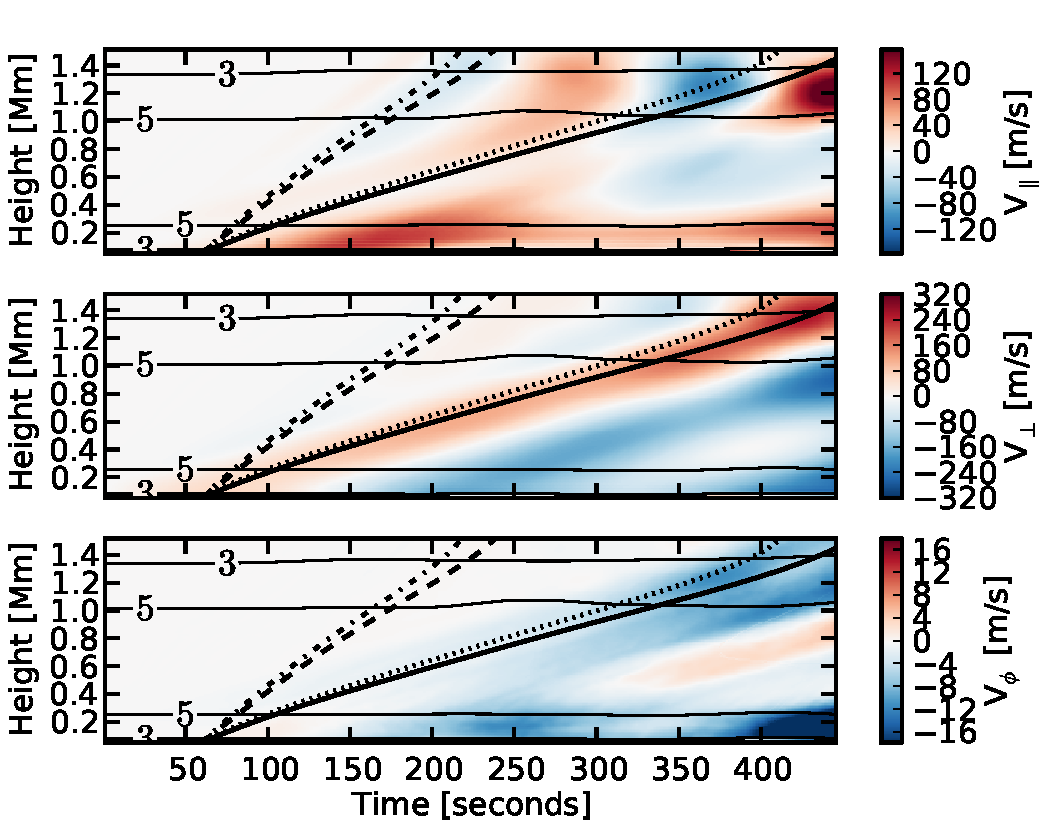
\includegraphics[width=\columnwidth]{Chapter4/Figs/TD_wave_speeds_horiz_p240_A10_r30.pdf}
        \caption{Horizontal Driver}
        \label{fig:All_TD_wave_30:horiz}
    \end{subfigure}
    \begin{subfigure}[b]{0.49\textwidth}
        \includegraphics[width=\columnwidth]{Chapter4/Figs/TD_wave_speeds_vert_p240_A10_r30.pdf}
        \caption{Vertical Driver}
        \label{fig:All_TD_wave_30:vert}
    \end{subfigure}
    
    \begin{subfigure}[b]{0.49\textwidth}
        \includegraphics[width=\columnwidth]{Chapter4/Figs/TD_wave_speeds_Suni_p240_A10_r30_B0.pdf}
        \caption{Uniform Torsional Driver}
        \label{fig:All_TD_wave_30:Suni}
    \end{subfigure}
    \begin{subfigure}[b]{0.49\textwidth}
        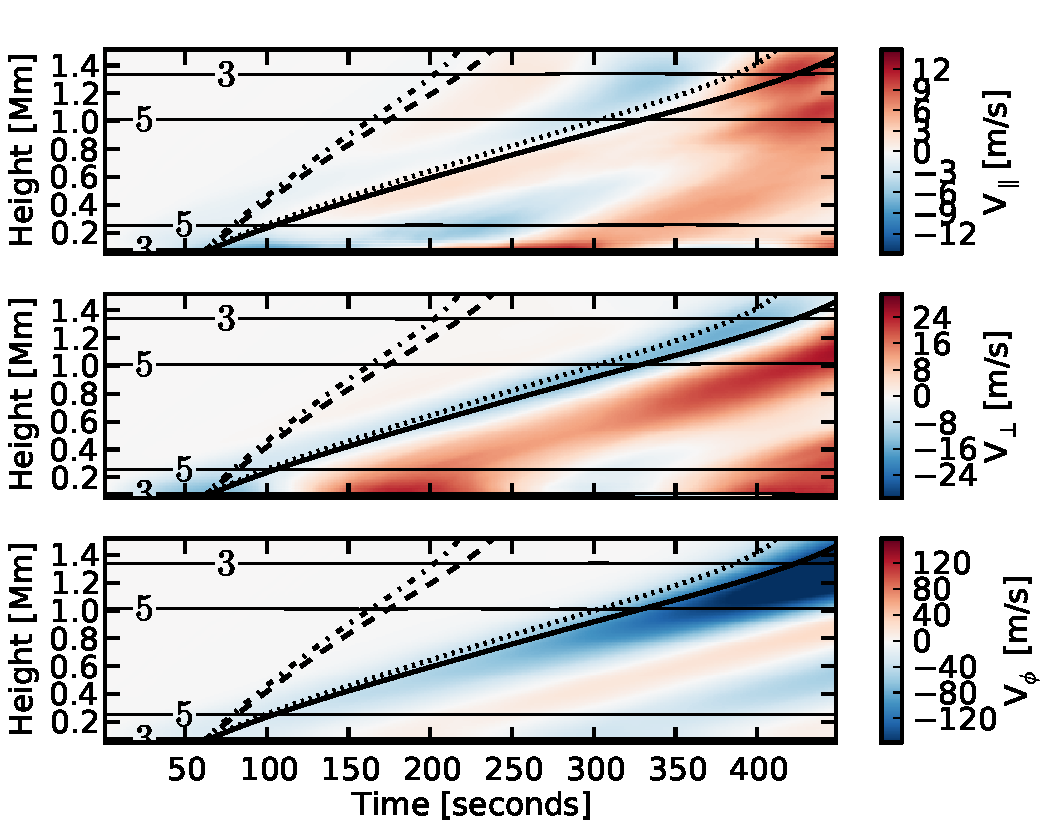
\includegraphics[width=\columnwidth]{Chapter4/Figs/TD_wave_speeds_Sarch_p240_A10_r30_B0005.pdf}
        \caption{Archimedean Spiral Type Driver}
        \label{fig:All_TD_wave_30:Sarch}
    \end{subfigure}
    
    \begin{subfigure}[b]{0.49\textwidth}
        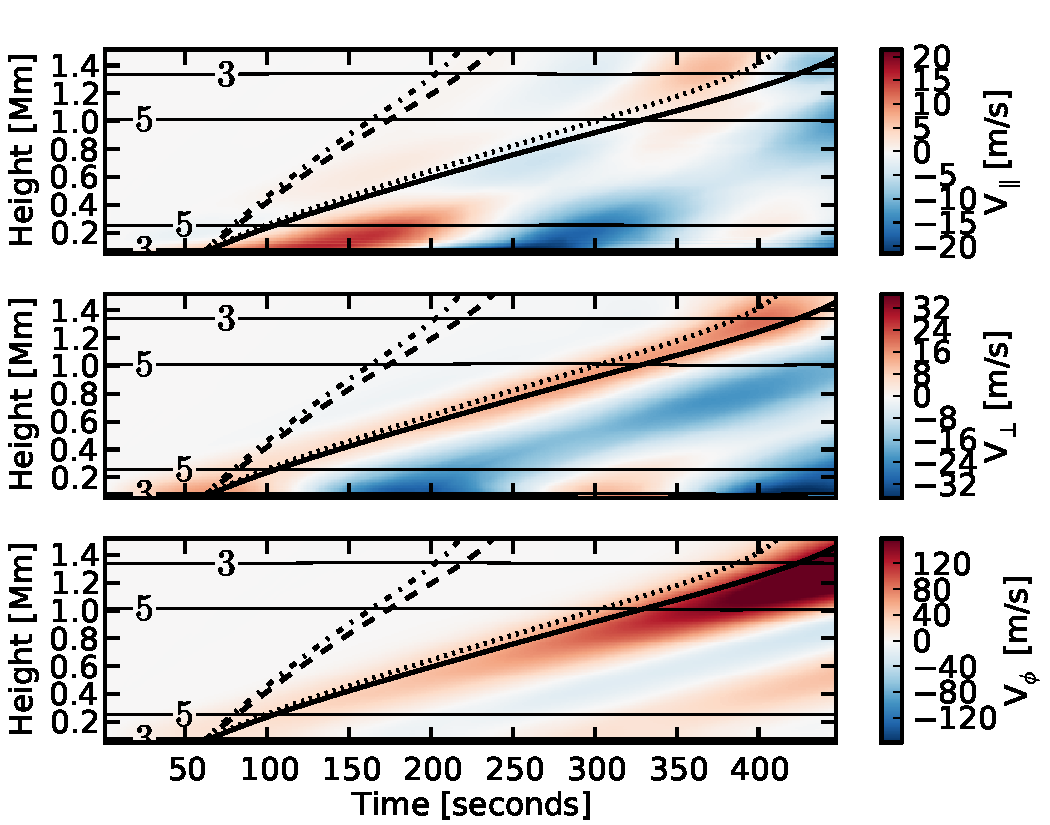
\includegraphics[width=\columnwidth]{Chapter4/Figs/TD_wave_speeds_Slog_p240_A10_r30_B005.pdf}
        \caption{Logarithmic Spiral Type Driver}
        \label{fig:All_TD_wave_30:Slog}
    \end{subfigure}
    \caption{Decomposed velocity perturbation time-distance diagrams along the flux surface at radius $r = 468$ km (approximately central in the magnetic flux tube) for all simulated drivers. Horizontal black lines are plasma-$\beta$ contours, over-plotted are characteristic background speeds, the dot-dashed line is the fast speed ($v_f$), the dashed line is the sound speed ($c_s$), the dotted line is the Alfv\'en speed ($v_A$) and the solid line is the slow speed ($v_t$).}
    \label{fig:All_TD_wave_30}
\end{figure*}

\subsection{Wave Energy Flux}\label{sec:energy_flux}

\begin{figure*}
    \centering
    \begin{subfigure}[b]{0.49\textwidth}
        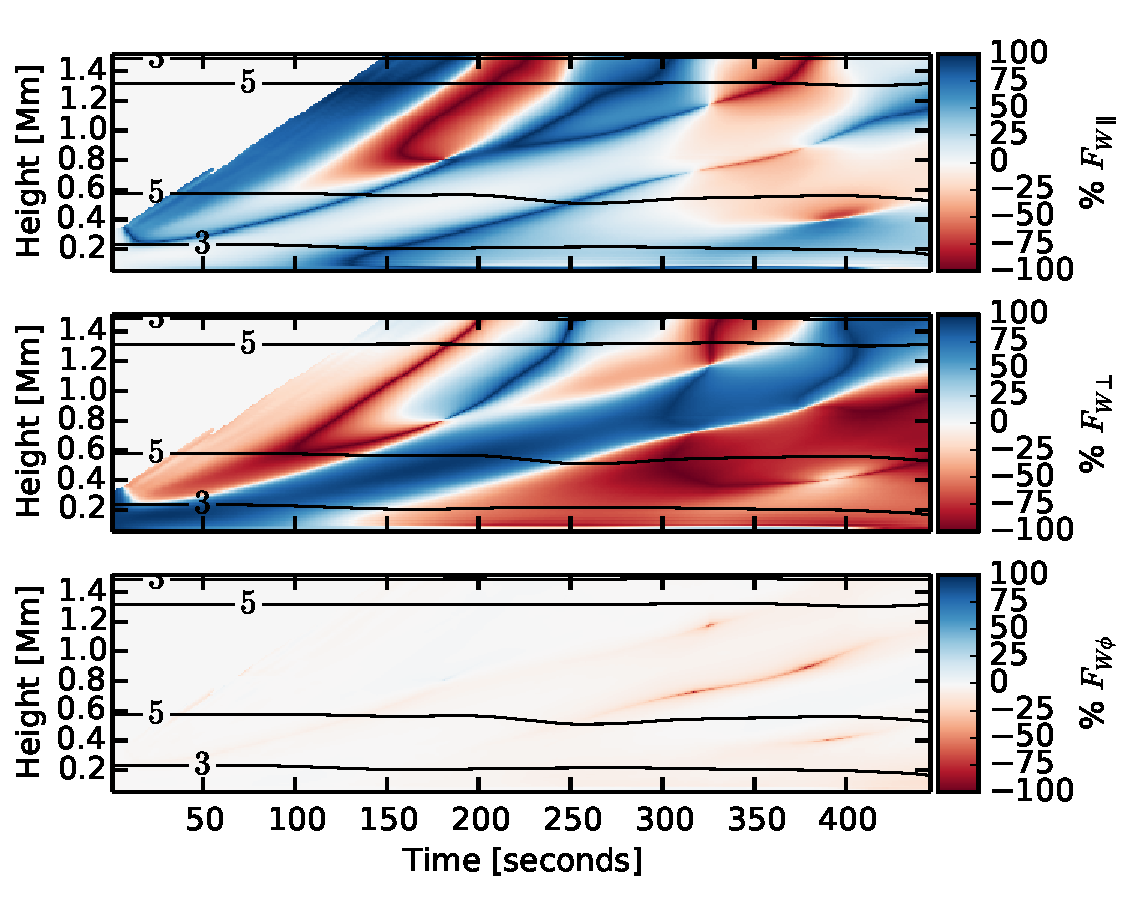
\includegraphics[width=\columnwidth]{Chapter4/Figs/WaveFlux_TD_Percent_horiz_p240_A10_r30.pdf}
        \caption{Horizontal Driver}
    \end{subfigure}
    \begin{subfigure}[b]{0.49\textwidth}
        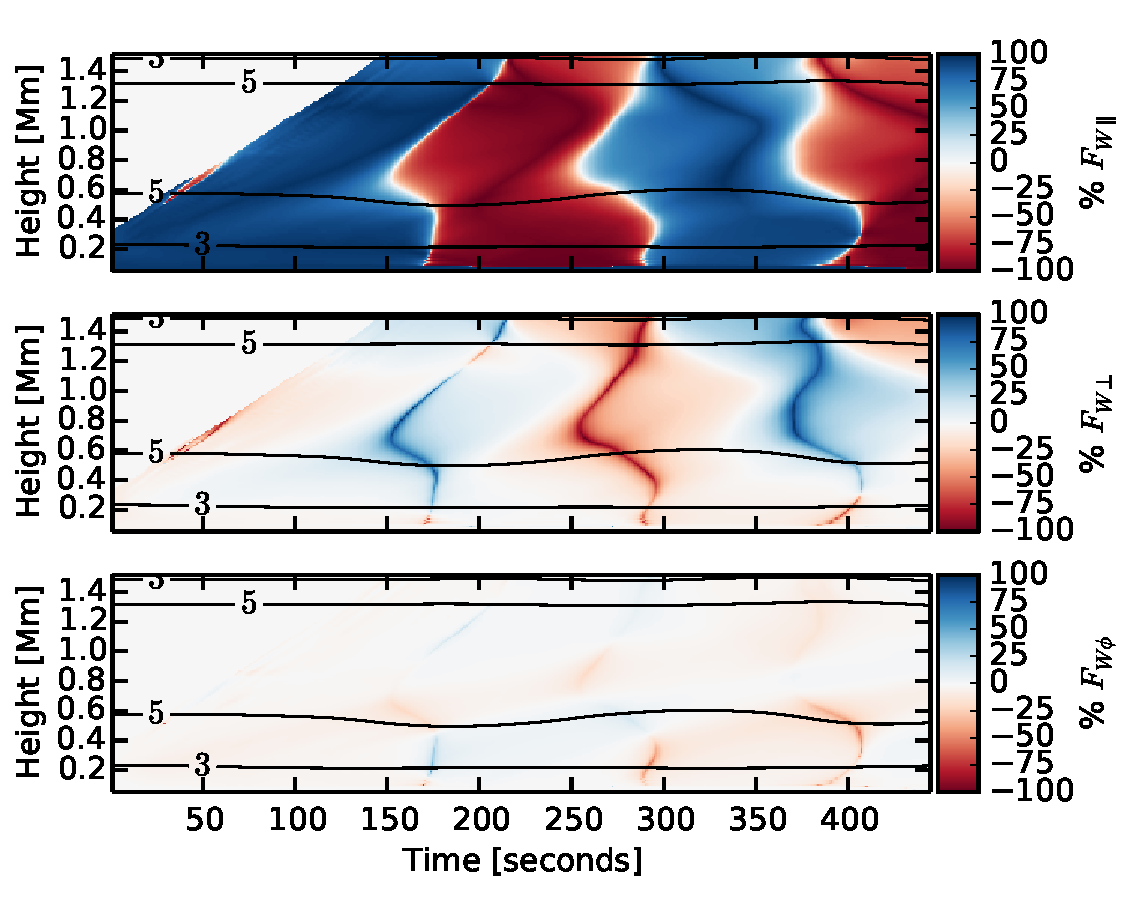
\includegraphics[width=\columnwidth]{Chapter4/Figs/WaveFlux_TD_Percent_vert_p240_A10_r30.pdf}
        \caption{Vertical Driver}
    \end{subfigure}
    
    \begin{subfigure}[b]{0.49\textwidth}
        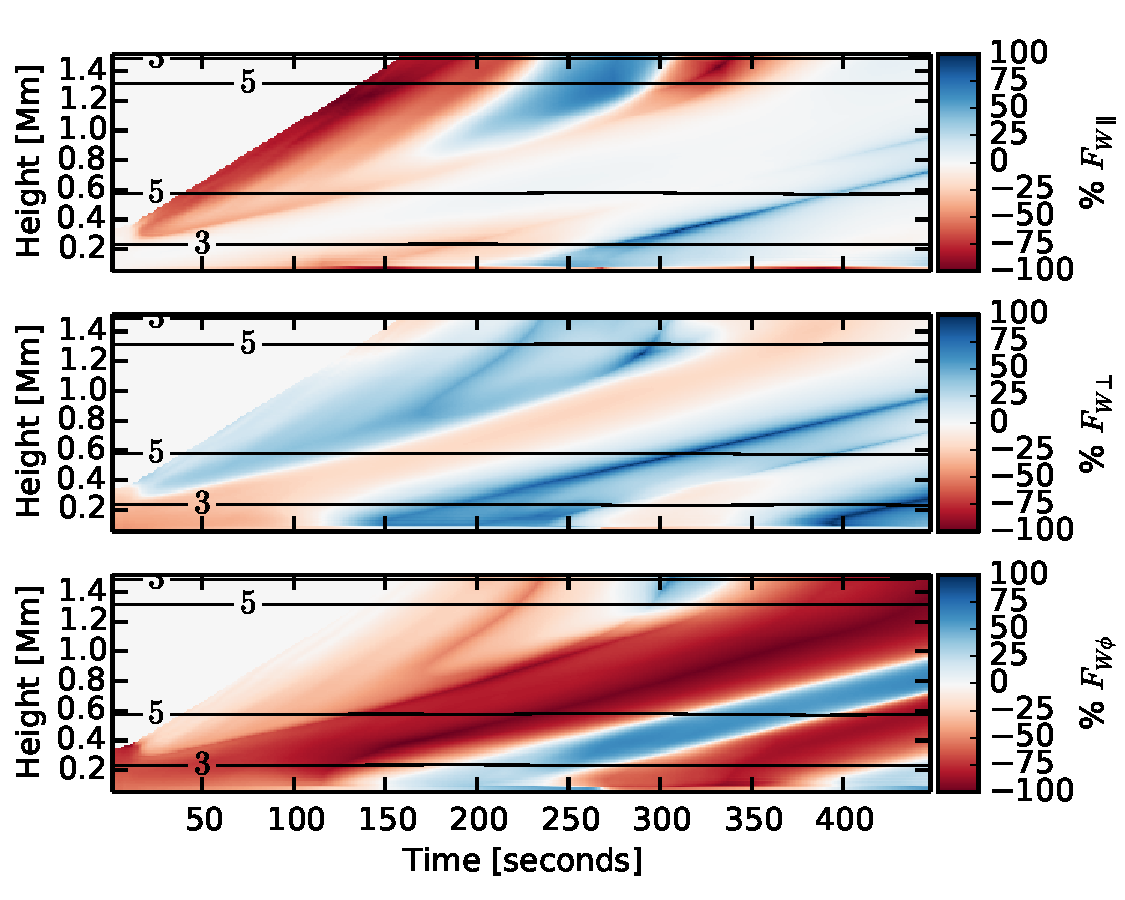
\includegraphics[width=\columnwidth]{Chapter4/Figs/WaveFlux_TD_Percent_Suni_p240_A10_r30_B0.pdf}
        \caption{Uniform Torsional Driver}
    \end{subfigure}
    \begin{subfigure}[b]{0.49\textwidth}
        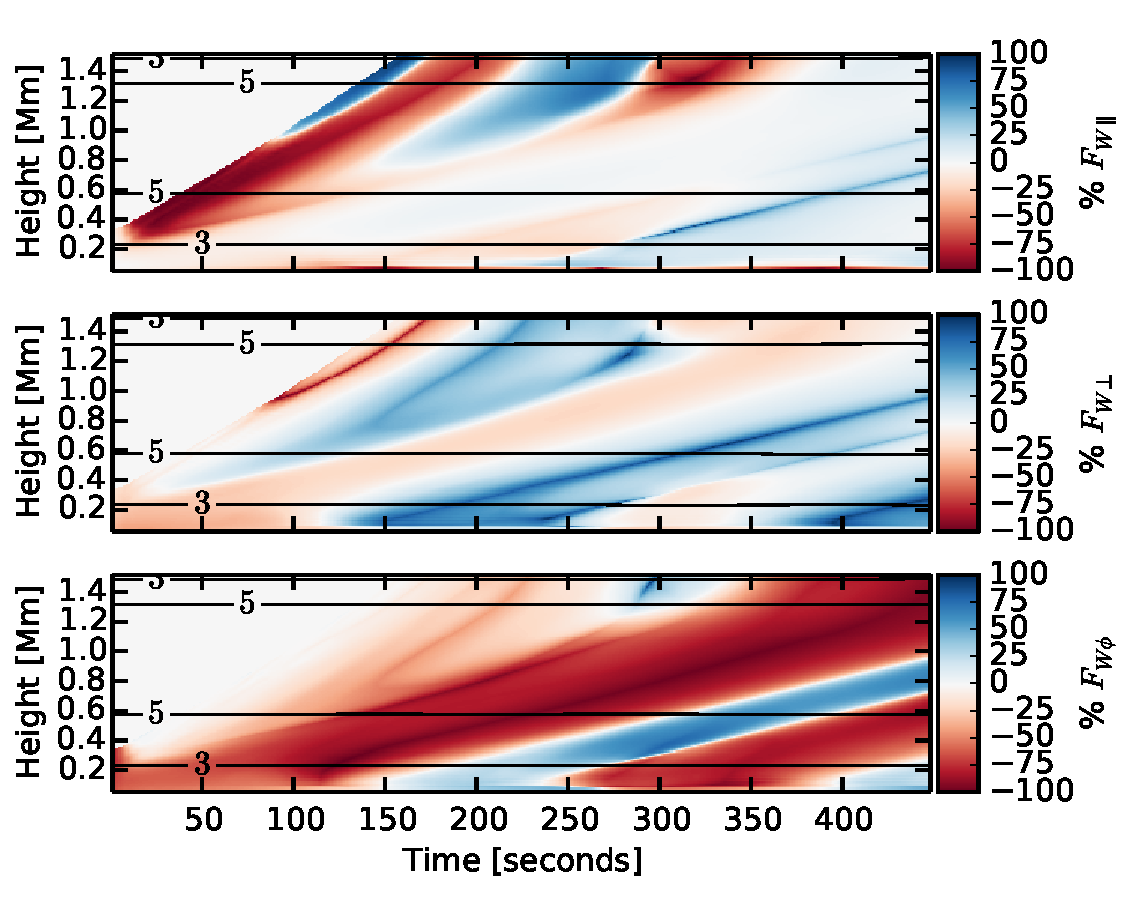
\includegraphics[width=\columnwidth]{Chapter4/Figs/WaveFlux_TD_Percent_Sarch_p240_A10_r30_B0005.pdf}
        \caption{Archimedean Spiral Type Driver}
    \end{subfigure}
    
    \begin{subfigure}[b]{0.49\textwidth}
        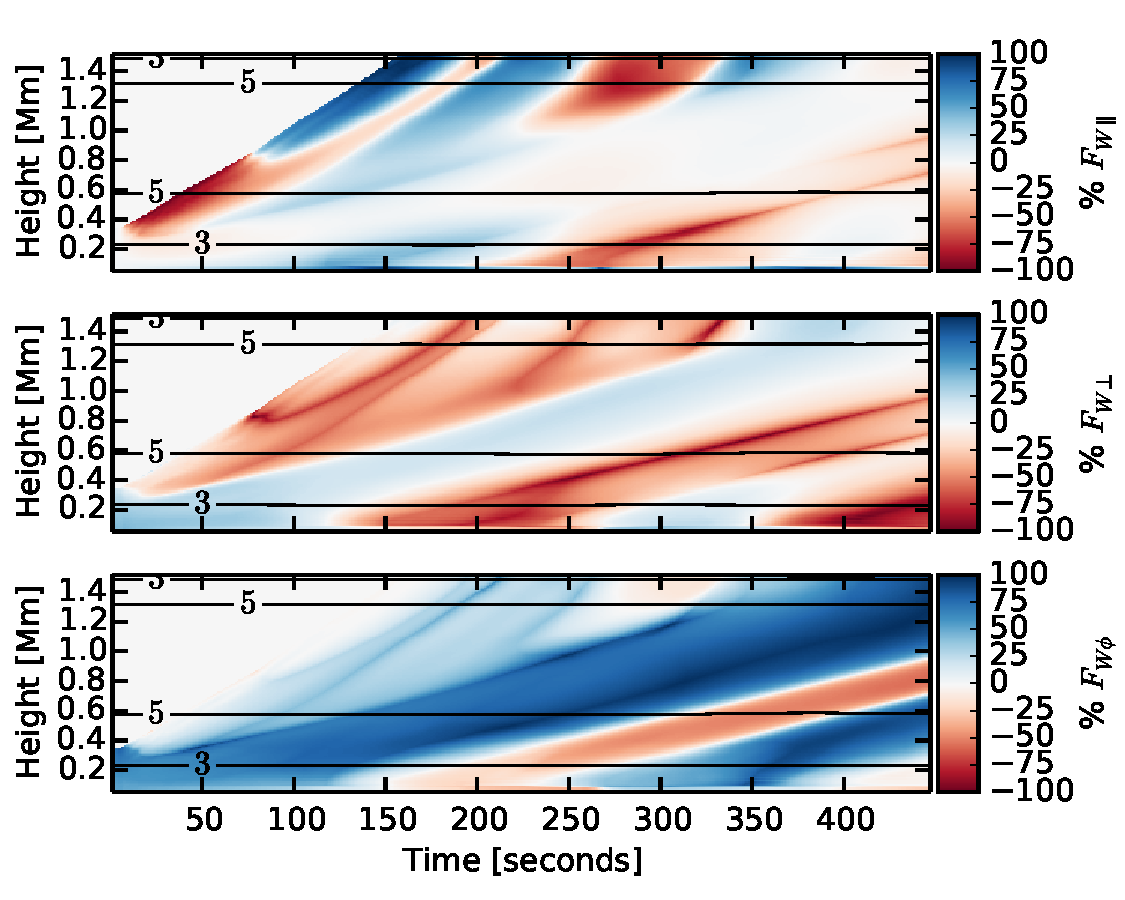
\includegraphics[width=\columnwidth]{Chapter4/Figs/WaveFlux_TD_Percent_Slog_p240_A10_r30_B005.pdf}
        \caption{Logarithmic Spiral Type Driver}
    \end{subfigure}
    \caption{Decomposed wave energy flux time-distance diagrams along the flux surface at radius $r = 468$ km (approximately central in the flux tube) for all simulated drivers. The three components of Energy flux ($F_\parallel$, $F_\perp$ and $F_\phi$) are calculated, then, the proportion for each component is shown for a strip up the flux surface.}
    \label{fig:All_Flux_percent_TD}
\end{figure*}

To calculate the relative strengths of the excited waves we compute the `wave energy flux' vector everywhere in the domain using Equation \ref{eq:wave_energy}.
\begin{equation}
\vec{F}_{wave} \equiv \widetilde{p}_k \vec{v} + \frac{1}{\mu_0} \left(\vec{B}_b \cdot \vec{\widetilde{B}}\right) \vec{v} - \frac{1}{\mu_0}\left(\vec{v} \cdot \vec{\widetilde{B}} \right) \vec{B}_b,
\label{eq:wave_energy}
\end{equation}
where a subscript $b$ represents a background variable, a tilda represents a perturbation from the background conditions and $p_k$ represents kinetic pressure.

This equation has been widely used to calculate the energy contained in linear MHD perturbations.
It is discussed in detail in \cite{bogdan2003} where it is compared to the `true' MHD flux for linear perturbations and found to be generally clearer. 
It is used in \cite{vigeesh2009, vigeesh2012, khomenko2012}. 
For a full derivation and discussion relating to time-averaging see \cite{leroy1985}.
Calculating wave energy flux using Equation \ref{eq:wave_energy} provides a vector which is useful in plotting time distance diagrams and analysing wave modes.
However, when averaging it to compute the values used in Figure \ref{fig:flux_bar_graph} the nature of the wave energy flux means that if there are standing waves in the domain the fluxes would cancel and therefore under represent the amount of energy excited into that component.
While it is not expected to find standing waves in these simulations, we use Equations \ref{eq:flux_par} - \ref{eq:flux_phi} below, from \citet{vigeesh2012} and \citet{khomenko2012} to calculate the average `available' energy flux.
These equations give an estimate of the `available' flux as energy density multiplied by wave speed.
Which is advantageous for calculating the total average as it results in a positive value that is not negated by standing waves.

\begin{align}
F_\parallel = \rho v_\parallel^2 c_s,\label{eq:flux_par}\\
F_\perp = \rho v_\perp^2 v_A,\label{eq:flux_perp}\\
F_\phi = \rho v_\phi^2v_A.\label{eq:flux_phi}
\end{align}
here, $F_\parallel$, $F_\perp$ and $F_\phi$ are the parallel, perpendicular and azimuthal components of energy flux respectively.

Once the wave energy flux has been computed, it is decomposed into parallel, perpendicular and azimuthal components using the same method as the velocity vector. 
Using the analysis method outlined in Section \ref{sec:3d_analysis} time-distance diagrams are computed for the percentage wave energy flux (see Fig. \ref{fig:All_Flux_percent_TD}). 
The percentage values are plotted to highlight the relative strengths of the excited wave modes, and to enable a comparison of which modes are dominant. 
The absolute average energy flux over all heights is summed for all times for each component.

\begin{figure}
    \centering
    \includegraphics[width=0.7\columnwidth]{Chapter4/Figs/p240_A10_Wave_Flux_comparision.pdf}
    \caption{Percentage total available energy flux comparison (calculated using Equations \ref{eq:flux_par} - \ref{eq:flux_phi}), for all drivers and all flux surfaces. The $F_\parallel$ component is shown as green, the $F_\perp$ component is shown in red and the $F_\phi$ component is shown in blue.}
    \label{fig:flux_bar_graph}
\end{figure}

By comparing Figs. \ref{fig:All_TD_wave_30} \& \ref{fig:All_Flux_percent_TD} we find that for the wave modes excited by the horizontal driver $60$\% of the energy flux is in the perpendicular component $F_\perp$ which is attributed to the slow kink mode.
The rest of the flux is in the parallel component $F_\parallel$. 
The vertical driver simulation has $79.3$\% of the energy flux in the $F_\parallel$ component, identified as the fast sausage mode, with the $F_\perp$ component only contributing $12.5$\%. 
The simulations with spiral drivers all have up to $60$\% of their energy flux in the azimuthal component $F_\phi$. 
The logarithmic spiral source excites a slightly higher percentage of the flux in the slow kink mode and the fast sausage mode, in comparison to the uniform torsional and Archimedean spiral driver.

The summarised energy flux results, and their equivalents for different flux tube radii are shown in Fig. \ref{fig:flux_bar_graph}.
With reasonable accuracy we can attribute each of the energy flux components shown to one or two MHD wave modes.
The $F_\parallel$ component is generally the fast sausage mode. 
The $F_\perp$ component is almost exclusively excited by the slow kink mode.
Finally, the $F_\phi$ is attributed to the Alfv\'en mode.
Another interesting result is that the type of spiral driver used has a minimal impact upon the amount of flux in each wave mode (see Fig. \ref{fig:flux_bar_graph}).
This could be dependent upon the spiral expansion factor used in the logarithmic and Archimedean spirals, which could be the subject of a further parameter study.

\subsection{Flux Tube Radius}
The plasma properties vary within the computational domain due to the magnetic field configuration.
This also means that the wave propagation on the surface of a flux tube is dependent upon its radius. 
We define the radius of the flux tube at the top of the domain and as its initial radius.
There are an arbitrary number of definable flux tube surfaces in our domain as defined from the top outer edge of the domain inwards. 
To demonstrate the difference in propagation caused by the change in plasma properties, especially $\beta$, with a change in radii we have computed all the analysis for three different flux tubes, with radii of $r=936$ km, $r=468$ km and  $r=156$ km; These radii are chosen to represent a good spectrum across the domain.

The results of the flux calculations are summarised in Fig. \ref{fig:flux_bar_graph}.
The smallest radius flux tube, shown in the top panel, shows that, for the torsional driver simulations, less azimuthal ($F_\phi$) flux is generated closer to the axis of the flux tube. 
This is expected due to a higher magnetic pressure towards the axis of the tube; the flux is, instead, excited evenly in the parallel ($F_\parallel$) and perpendicular ($F_\perp$) components as predominately kink and sausage modes. 
For higher radii surfaces the $F_\parallel$ component dominates the $F_\perp$ component; as the distance from the axis increases the influence of the kink mode decreases.
In the case of the horizontal and vertical drivers, most of the flux is excited in the slow kink and sausage modes respectively.
In the horizontal case, for the larger radius tube, the sausage mode, in the $F_\parallel$ component, again begins to dominate the kink mode, in the $F_\perp$ component.
